%APÊNDICES
\thispagestyle{empty}

\part*{Apêndices} % se quiser uma página indicativa de APÊNDICES antes dos apêndices.
%Caso não queira, comente a linha acima.
\addcontentsline{toc}{part}{Apêndices}
%Conforme a norma, os apêndices devem se organizar em ordem alfabética: A, B, C, D...
\chapterstyle{crosshead}
\chapter*{Apêndice A -- Um apêndice}
\addcontentsline{toc}{chapter}{Anexo A -- Um apêndice}

\begin{center}
	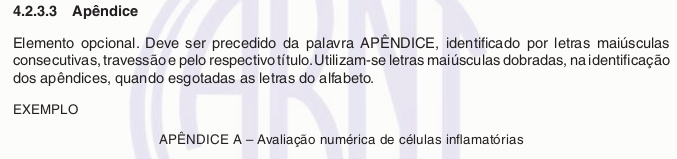
\includegraphics[scale=.60]{./img/apendice-img1.png}
\end{center}

\chapter*{Apêndice B -- Um outro apêndice}
\addcontentsline{toc}{chapter}{Anexo B -- Um outro apêndice}

\begin{center}
	
\includegraphics[scale=.60]{./img/apendice-img.png}
\end{center}


%================================================
%ANEXOS
\thispagestyle{empty}
\part*{Anexos} % Se quiser uma página indicativa de ANEXOS antes dos anexos.
%Caso não queira, comente a linha acima.
\addcontentsline{toc}{part}{Anexos}
%Conforme a norma, os anexos devem se organizar em ordem alfabética: A, B, C, D...
\chapterstyle{crosshead}
\chapter*{Anexo A -- Um anexo}
\addcontentsline{toc}{chapter}{Anexo A -- Um anexo}

\begin{center}
	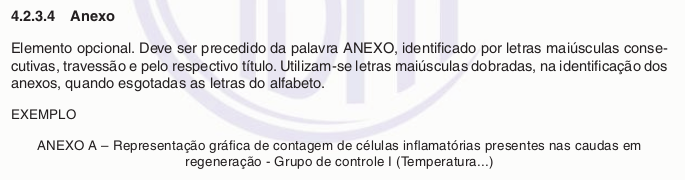
\includegraphics[scale=.60]{./img/anexo-img1.png}
\end{center}

\chapter*{Anexo B -- Um anexo}
\addcontentsline{toc}{chapter}{Anexo B -- Um outro anexo}

\begin{center}
	
\includegraphics[scale=.60]{./img/anexo-img.png}
\end{center}


